% 5. Prototyp (Implementierung, Patterns, Tests)
\chapter{Implementing the Modular Proxy Application}
\label{chap:implementation}
This chapter covers an exemplaric implementation of the concept that was worked out in chapter \ref{chap:conceptual-design}, starting with formally describing the goals and constraints of this implementation in section \ref{sec:goals-constraints}. Afterwards, an overview and comparison of available and suitable tools for the task is performed in section \ref{sec:tool-selection}. The chapter concludes with details about the implementation of individual components in section \ref{sec:individual-components}, describing how specific challenges were overcome.% and what design patterns were used.

\section{Goals and Constraints}
\label{sec:goals-constraints}
The goal of this thesis' implementation was to implement the \enquote{Monolithic Proxy Application} design concept described in section \ref{sec:design-1} to a maturity level that allowed to test its usefulness and effectiveness in the testbed described in section \ref{sec:prototype-testing}. Thus, a focus was set on implementing a vertical prototype that featured important core components (such as factories, state-machines and network stacks) and a set of exemplaric protocol implementations (\ac{HTTP}, \ac{WS} and \ac{MQTT}). Similar to the first prototype discussed in section \ref{sec:prototypical-implementation}, this prototype was a proof-of-concept implementation and neglected quality attributes such as usability and performance.\\
The prototype had the working title \enquote{net-riot}, which indicated that this was a networking tool and was to be used in the \ac{IoT} context. While its core components and protocol implementations were successfully implemented and worked individually, the interaction between protocol implementations at runtime failed and could not be resolved before the end of this thesis.

\section{Tool Selection}
\label{sec:tool-selection}
To choose the tools for implementing the design concept, a list of requirements to tools was inferred from the software requirements discussed and expert interviews shown in chapter \ref{chap:understanding-the-problem-space}:
\begin{itemize}
    \item [\textbf{F1}] \textbf{Scripting:} The tool must provide scripting capabilities that allow penetration testers to execute complex scripted operations on messages.
    \item [\textbf{F2}] \textbf{Libraries:} In order to avoid custom implementation of the \ac{HTTP}, \ac{WS} and \ac{MQTT} protocols, the tool must provide a rich set of libraries that can be used to work with said protocols.
    \item [\textbf{F3}] \textbf{Deployment:} To allow the prototype to be installed in an uncomplicated way, the tool must provide or support mechanisms that simplify deployment, such as code compilation and static linking of dependencies or containerization.
    \item [\textbf{F4}] \textbf{Accessibility:} The tool must be powerful and complex enough to solve the software requirements and implement the design concept, but it must also feature a \enquote{barrier or entry} that is low enough so extending the application is feasible for open source developers.
\end{itemize}

It was found that Python satisfied all of these requirements:
\begin{itemize}
    \item Python is a free, open source and general purpose programming language that was first released in 1991 and is being continuously improved and updated. % 978-0-262-52962-4
    \item The built-in \emph{exec}\footnote{https://docs.python.org/3/library/functions.html\#exec} function provides execution of arbitrary Python code at runtime. Although it is infamous for its security implications, it is very suitable for scripting.
    \item The \ac{PyPI} is a public repository of more than 300.000\footnote{Based on \ac{PyPI}'s statistics: https://pypi.org/} Python packages that can be installed using the \emph{pip} command-line tool. There are numerous packages that implement the protocols \ac{WS}, \ac{MQTT} and \ac{HTTP}.
    \item Python supports multiple ways to deploy projects, including packaging projects into executable files \footnote{https://packaging.python.org/overview/\#bringing-your-own-python-executable} and containerization\footnote{e.g. using Docker https://hub.docker.com/\_/python/}.
    \item Its comparatively simple syntax and its design philosophy that values accessible code higher than performance\footnote{Described in 19 aphorisms in \enquote{The Zen of Python} (https://www.python.org/dev/peps/pep-0020/)} encourage readability and maintainability in Python projects. When implemented, this makes Python an accessible programming language. Also, its optional static typing allows to omit redundant type information for simple methods and to provide explicit type information for complex and shared pieces of code like algorithms and interfaces.
\end{itemize} %TODO: Python is free?
Git was used for version-control and Microsoft Visual Studio Code was the \ac{IDE} used for implementation.

\begin{figure}[h]
    \centering
    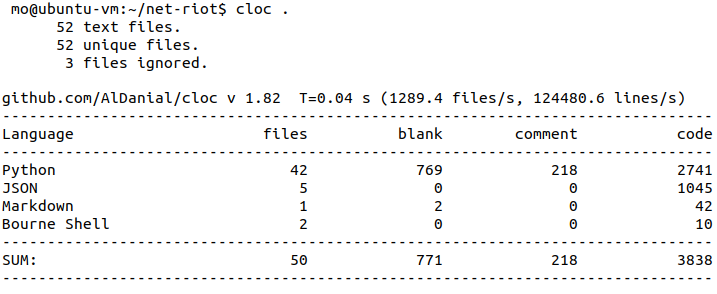
\includegraphics[width=12cm]{img/ch06/cloc.png}
    \captionof{figure}{?} %TODO: Describe
    \label{fig:cloc}
\end{figure}


\section{Individual Components}
\label{sec:individual-components}

\subsection{Network Stack}
\subsubsection{Gateways}
The protocols used in scenario \#2 that net-riot was implemented for were using \ac{TCP} for transport. Therefore, net-riot implemented a \ac{TCP}-Gateway that allowed it to create \ac{TCP} server sockets to listen on for incoming connection requests. For incoming connections C\textsubscript{I}, respective outgoing connections C\textsubscript{O} were initialized and connected to a preconfigured remote server. For each of those connections, \enquote{TcpPipe} instances P\textsubscript{I} and P\textsubscript{O} were initialized that ran in separate threads and accepted incoming packets. The gateway then initialized \enquote{TcpGatewayPipe} instances with P\textsubscript{I} and P\textsubscript{O} that routed messages originating from the TcpPipes into the pipeline and from the pipeline to the correct TcpPipe instance.
% TCP Gateway

\subsubsection{Encoders}
% Libraries used

\subsubsection{Scripting}
% Exec?
%\subsubsection{Pipelines}

\subsection{Configuration Parsing and Building}
\subsubsection{JSON Configuration and Schemas}
% Schema: definitions, flat hierarchy
\subsubsection{Factories, Builders and Templates}
% Site + NetRiotConfig + Templates + Reflection